	\newpage

	\section{Sprinty}

	\subsection{Sprint 1}

\subsubsection{Zadania do wykonania}

\begin{itemize}
	\item Logowanie i Rejestracja użytkowników
\end{itemize}

\subsubsection{Wykonane zadania}
\begin{itemize}
	\item Setup projektu, skonfigurowanie kontenerów Dockerowych
	\item Dodanie Rejestracji, logowania i wylogowywania użytkowników
\end{itemize}

\begin{figure}[H]
	\centering
	
\includegraphics[width=1\textwidth]{images/main_page.png}
	\caption{\centering{Strona główna}}
\end{figure}

\begin{figure}[H]
	\centering
	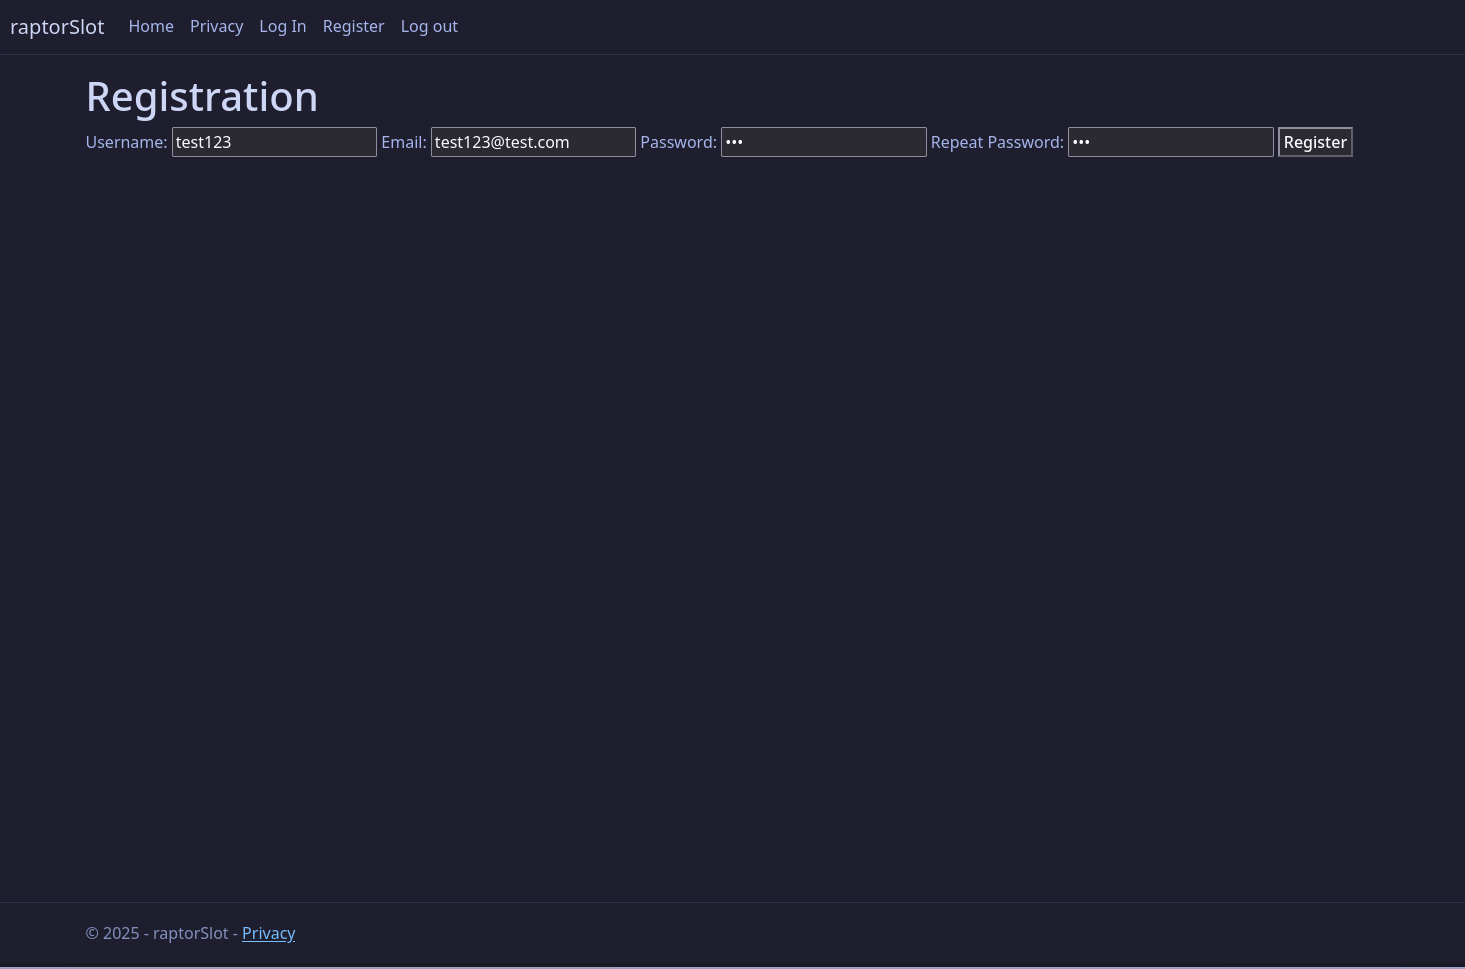
\includegraphics[width=1\textwidth]{images/register.png}
	\caption{\centering{Rejestracja}}
\end{figure}

\begin{figure}[H]
	\centering
	
\includegraphics[width=1\textwidth]{images/after_register.png}
	\caption{\centering{Po rejestracji}}
\end{figure}

\begin{figure}[H]
	\centering
	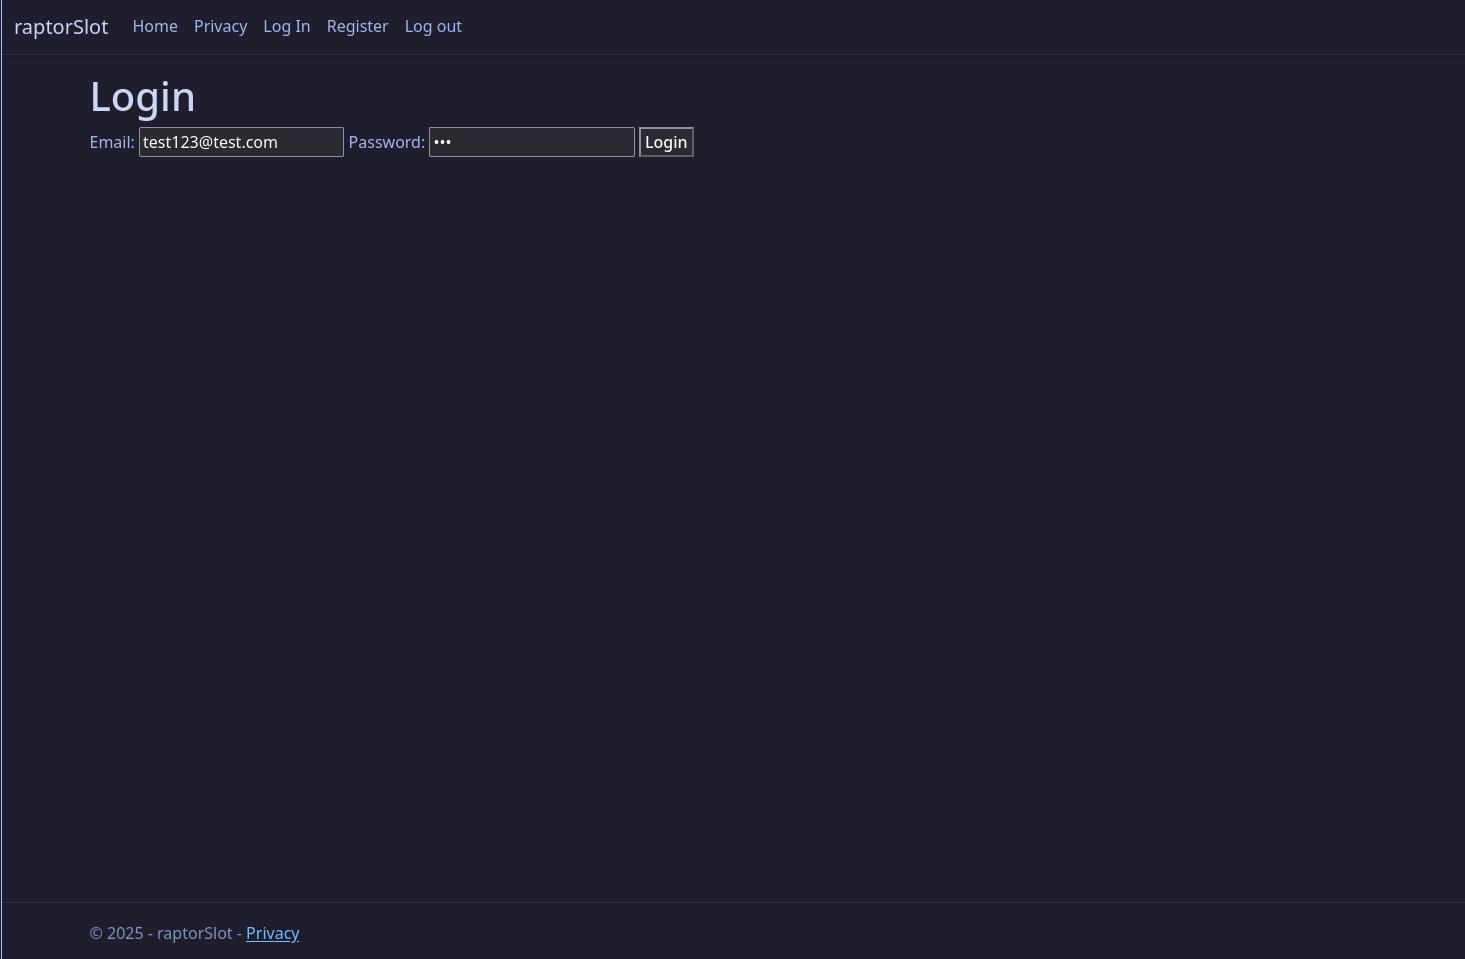
\includegraphics[width=1\textwidth]{images/login.png}
	\caption{\centering{Strona z loginem}}
\end{figure}
\subsubsection{Niewykonane zadania}

\begin{itemize}
\item Brak
\end{itemize}

\subsubsection{Napotkane problemy}

\begin{itemize}
\item Brak
\end{itemize}

\subsubsection{Zadania na kolejny tydzień}
\begin{itemize}
\item Kupowanie żetonów
\item Panel Administratora

\subsection{Sprint 2}


\subsubsection{Zadania do wykonania}

\begin{itemize}
	\item Panel Administratora
	\item Kupowanie żetonów zwykłych
\end{itemize}

\subsubsection{Wykonane zadania}
\begin{itemize}
	\item Panel Administratora - operacje CRUD na użytkownikach
	\item Kupowanie żetonów
\end{itemize}

\subsubsection{Efekty}

\begin{figure}[H]
	\centering
	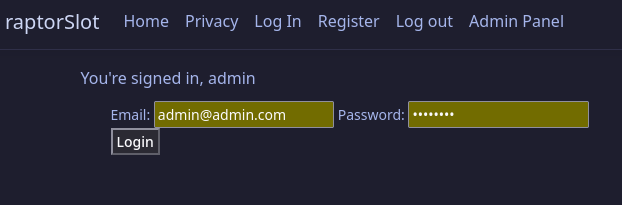
\includegraphics[width=1\textwidth]{images/admin_login.png}
	\caption{\centering{Logowanie na konto administratora}}
\end{figure}

\begin{figure}[H]
	\centering
	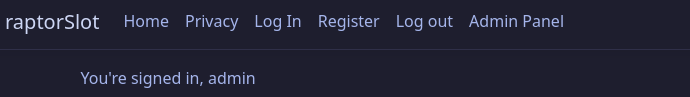
\includegraphics[width=1\textwidth]{images/admin_main.png}
	\caption{\centering{Główna strona administratora. Jest przejście do panelu}}
\end{figure}

\begin{figure}[H]
	\centering
	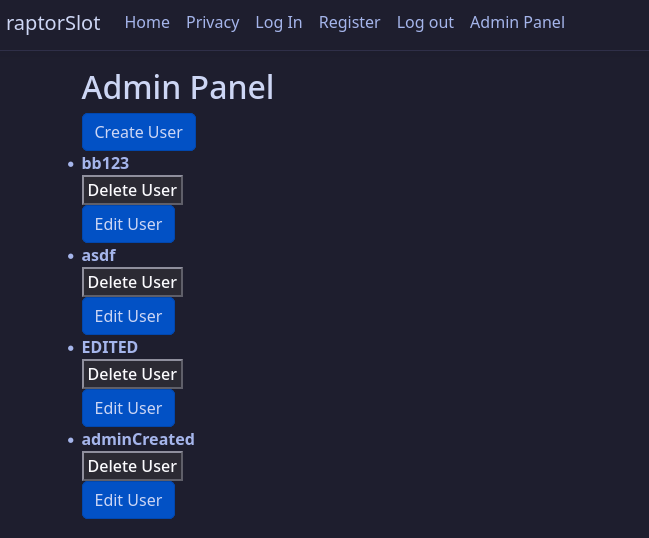
\includegraphics[width=1\textwidth]{images/admin_panel.png}
	\caption{\centering{Panel administratora}}
\end{figure}

\begin{figure}[H]
	\centering
	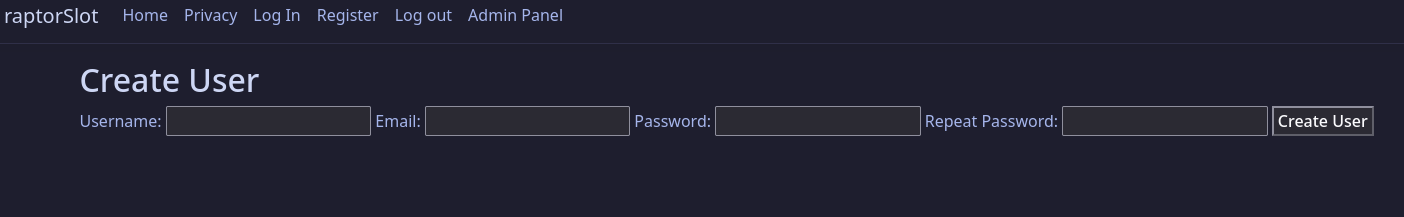
\includegraphics[width=1\textwidth]{images/admin_create.png}
	\caption{\centering{Tworzenie użytkownika}}
\end{figure}

\begin{figure}[H]
	\centering
	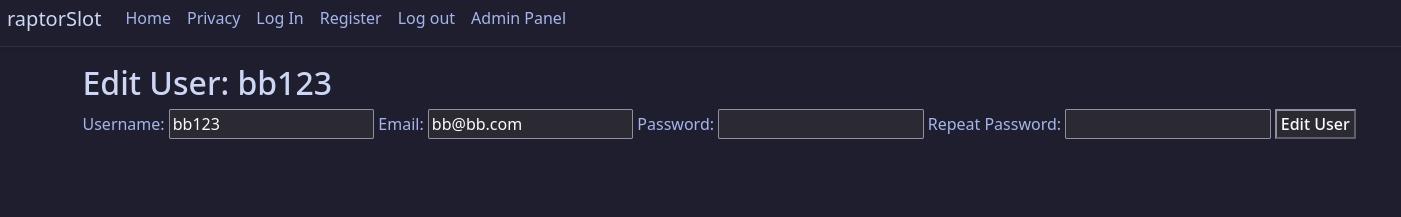
\includegraphics[width=1\textwidth]{images/admin_edit.png}
	\caption{\centering{Edytowanie użytkownika}}
\end{figure}

\begin{itemize}
\item Brak
\end{itemize}

\subsubsection{Napotkane problemy}

\begin{itemize}
\item Brak
\end{itemize}

\subsubsection{Zadania na kolejny tydzień}
\begin{itemize}
\item Stworzenie pierwszej gry - zgadywanie liczby
\item Losowanie żetonów premium w grach
\item Stworzenie Leaderboarda
\end{itemize}

\subsection{Sprint 3}

\subsubsection{Zadania do wykonania}

\begin{itemize}
    \item Stworzenie pierwszej gry - zgadywanie liczby
    \item Stworzenie drugiej gry - ruletka
    \item Losowanie żetonów premium w grach
    \item Stworzenie Leaderboarda
\end{itemize}

\subsubsection{Wykonane zadania}
\begin{itemize}
    \item Stworzenie pierwszej gry - zgadywanie liczby
    \item Stworzenie drugiej gry - ruletka
    \item Stworzenie Leaderboarda
\end{itemize}

\subsubsection{Efekty}

\begin{figure}[H]
    \centering
    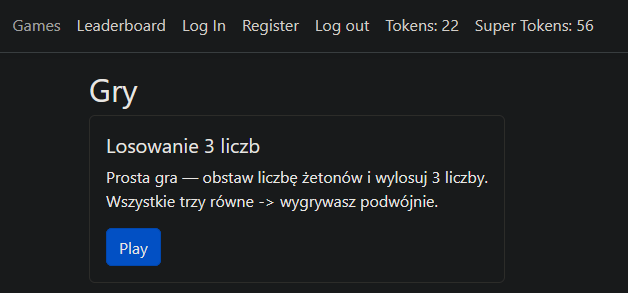
\includegraphics[width=0.75\linewidth]{images/numberdraw1.png}
    \caption{Widok menu wyboru gry dla losowania 3 liczb}
    \label{fig:numberdraw1}
\end{figure}

\begin{figure}[H]
    \centering
    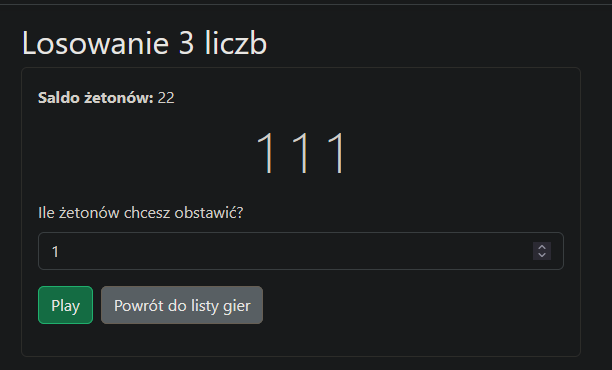
\includegraphics[width=0.75\linewidth]{images/numberdraw2.png}
    \caption{Widok gry losowania 3 liczb}
    \label{fig:numberdraw2}
\end{figure}

\begin{figure}[H]
    \centering
    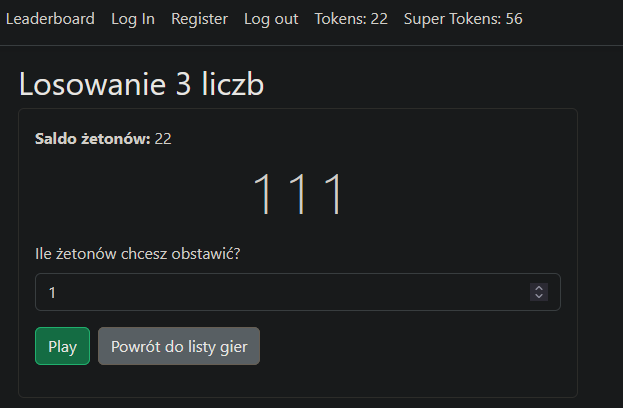
\includegraphics[width=0.75\linewidth]{images/numberdraw3.png}
    \caption{Wynik obstawienia 10 żetonów i kliknięcia play}
    \label{fig:numberdraw3}
\end{figure}

\begin{figure}[H]
    \centering
    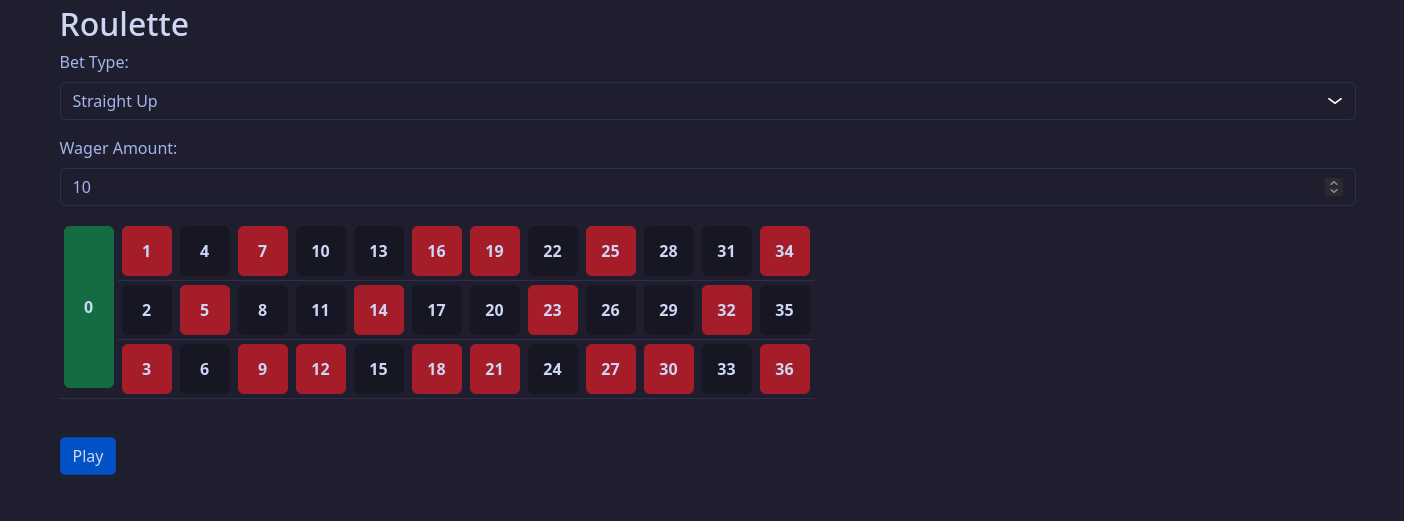
\includegraphics[width=0.75\linewidth]{images/roulete1.png}
    \caption{Widok gry ruletki}
    \label{fig:roulete1}
\end{figure}

\begin{figure}[H]
    \centering
    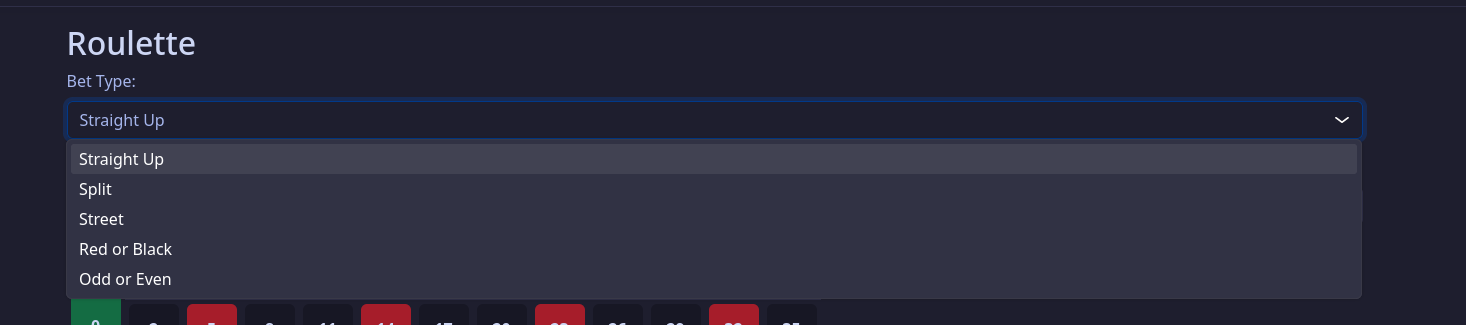
\includegraphics[width=0.75\linewidth]{images/roulete2.png}
    \caption{Widok na typy zakładów}
    \label{fig:roulete2}
\end{figure}

\begin{figure}[H]
    \centering
    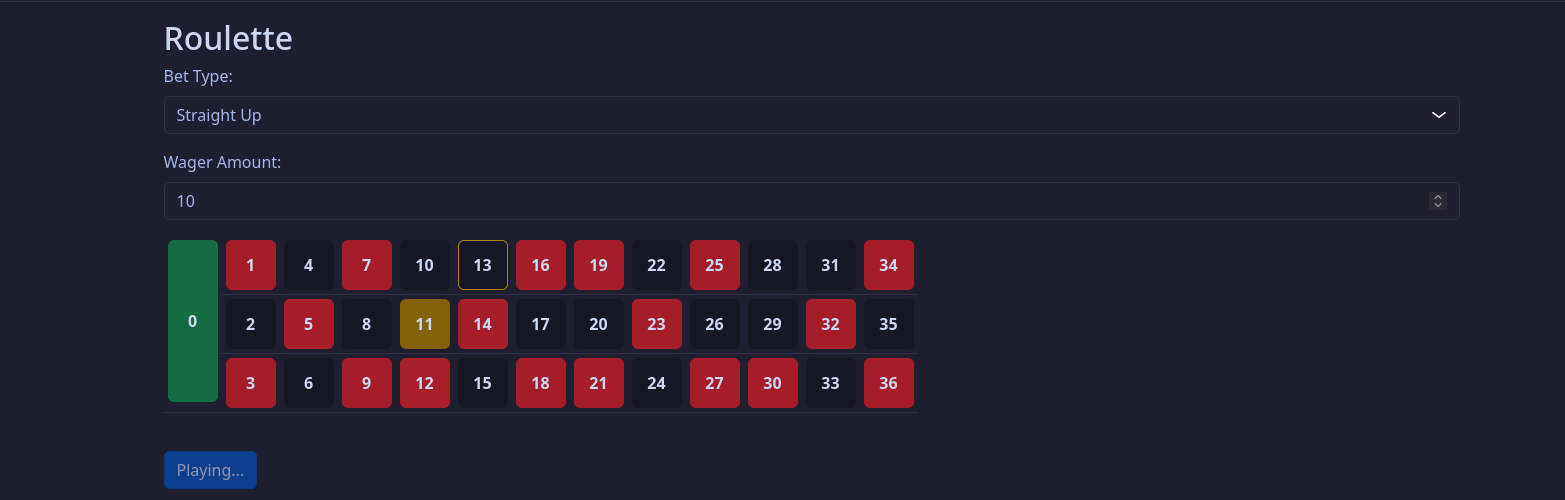
\includegraphics[width=0.75\linewidth]{images/roulete3.png}
    \caption{Widok na grę w trakcie losowania}
    \label{fig:roulete3}
\end{figure}

\begin{figure}[H]
    \centering
    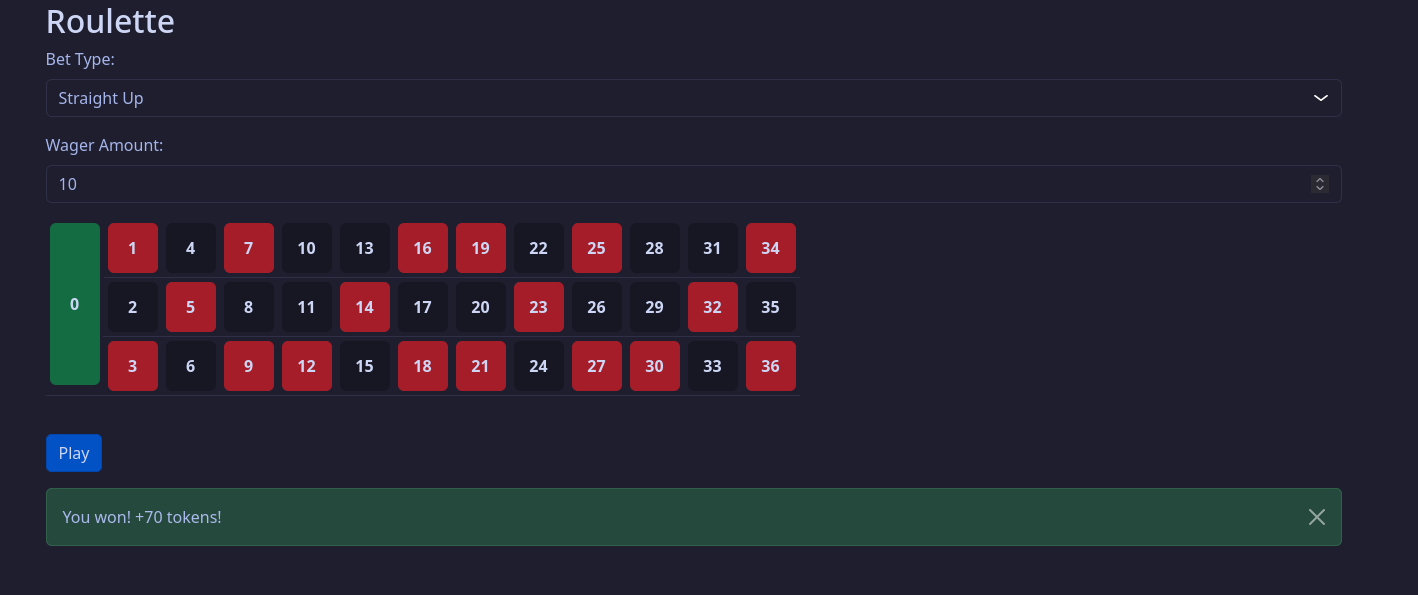
\includegraphics[width=0.75\linewidth]{images/roulete4.png}
    \caption{Widok na grę po wygranej}
    \label{fig:roulete4}
\end{figure}

\subsubsection{Niewykonane zadania}

\begin{itemize}
    \item Losowanie żetonów premium w grach
\end{itemize}

\subsubsection{Zadania na kolejny tydzień}
\begin{itemize}
    \item Dokończenie żetonów premium
    \item Napisanie 3 gry - obstawianie żetoów i liczby i porónanie z wylosowaną.
\end{itemize}

\subsection{Sprint 4}

\subsubsection{Zadania do wykonania}

\begin{itemize}
    \item Dokończenie żetonów premium
    \item Napisanie 3 gry - obstawianie żetoów i liczby i porónanie z wylosowaną.
\end{itemize}

\subsubsection{Wykonane zadania}
\begin{itemize}
    \item Dokończenie żetonów premium
    \item Napisanie 3 gry - obstawianie żetoów i liczby i porónanie z wylosowaną.
\end{itemize}

\subsubsection{Efekty}

\begin{figure}[H]
    \centering
    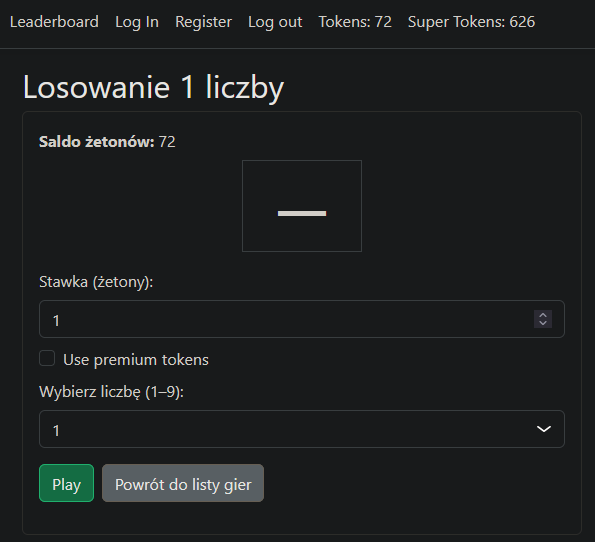
\includegraphics[width=0.75\linewidth]{images/3rdgameintlook.png}
    \caption{Widok interfejsu 3 gry - losowanie liczby i porównanie jej z wybraną}
    \label{fig:3rdgameintlook.png}
\end{figure}

\begin{figure}[H]
    \centering
    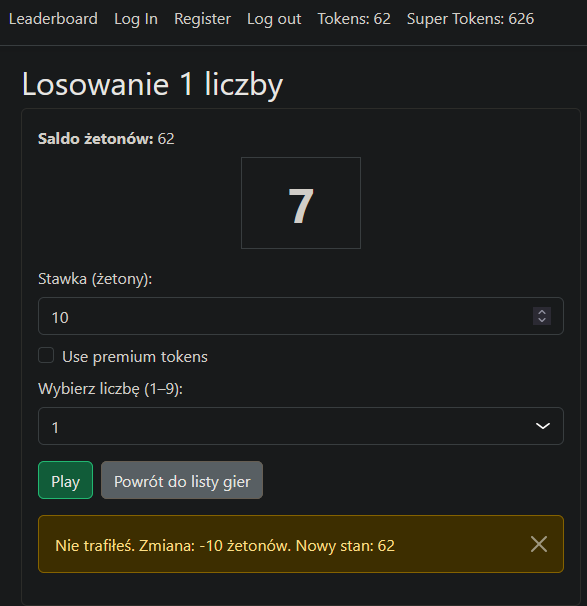
\includegraphics[width=0.75\linewidth]{images/3rdgameoutcome.png}
    \caption{Widok przegranej w 3 grze}
    \label{fig:3rdgameoutcome}
\end{figure}

\begin{figure}[H]
    \centering
    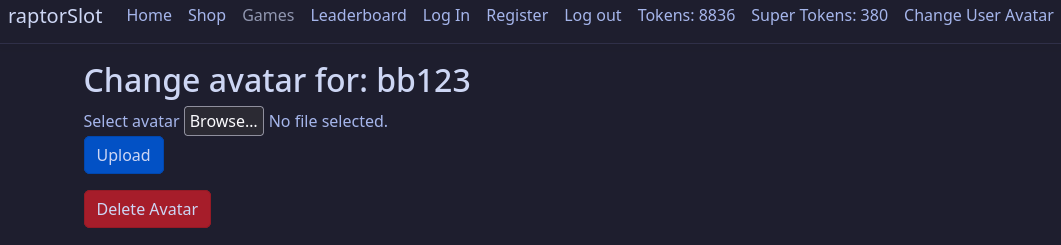
\includegraphics[width=0.75\linewidth]{images/Avatarview.png}
    \caption{Widok interfejsu wyboru awatara}
    \label{fig:Avatarview.png}
\end{figure}

\begin{figure}[H]
    \centering
    
\includegraphics[width=0.75\linewidth]{images/Avatarafteradd.png}
    \caption{Widok po dodaniu awatara}
    \label{fig:Avatarafteradd}
\end{figure}

\begin{figure}[H]
    \centering
    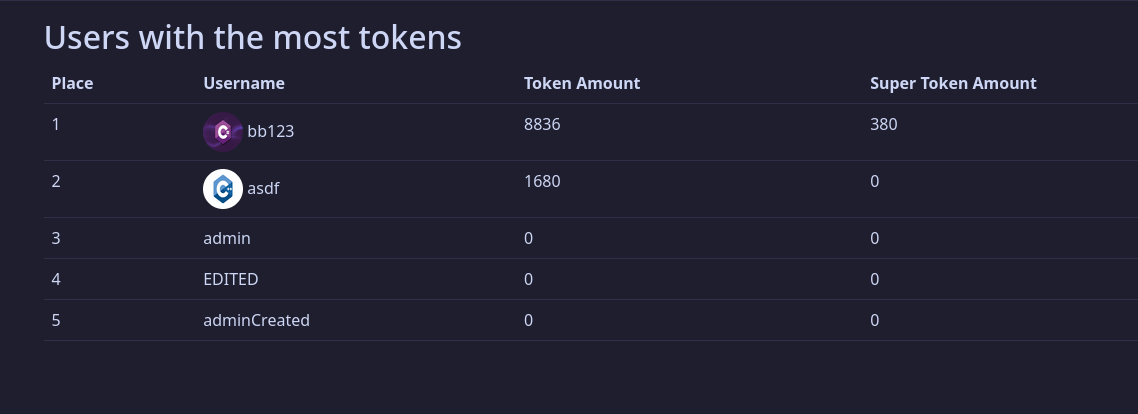
\includegraphics[width=0.75\linewidth]{images/Avatarviewleaderboard.png}
    \caption{Widok na tablice wyników z zaimplementowanym awatarem}
    \label{fig:Avatarviewleaderboard}
\end{figure}


\subsubsection{Niewykonane zadania}

\begin{itemize}
    \item Brak
\end{itemize}

\subsubsection{Zadania na kolejny tydzień}
\begin{itemize}
    \item Rozpoczęcie pracy nad dokumentacją
\end{itemize}
